\chapter{Results}

We discuss the results obtained using the tool through a number of real world cases.
The first of these additionally serves as a comprehensive, didactic, example of how to use the tool. 

\section{Diagnosing a failing inspection test in \mono{Text}}

Hearkening back to \mono{inspection-testing} discussed in \cref{section:introduction_inspection_testing}, we put
ourselves in the shoes of a programmer who gets surprised by a failing inspection test and reason how we might
employ HsComprehension to diagnose the problem. 

To summarize, we expected that the function \mono{countChars} which counts the number of characters in a \mono{ByteString}
using a number of functions in the \mono{Text} library, will in its final form not actually construct a \mono{Text} value.

\paragraph{1. Isolate the problem}
Modules typically contain more than 1 function and during the core2core transformations many more auxiliary functions are
added, and many functions are inlined to produce exponentially more code. Despite the tool being designed with features to 
comprehend medium-sized modules, it is still most helpful to temporarily isolate the
failing test case into a separate module:

\begin{minted}{haskell}
{-# LANGUAGE TemplateHaskell #-}

module InspectionTests where

import Test.Inspection
import qualified Data.Text as T
import qualified Data.Text.Encoding as TE
import Data.ByteString

countChars :: ByteString -> Int
countChars = T.length . T.toUpper . TE.decodeUtf8

-- the failing test case
inspect $ 'countChars `hasNoType` ''T.Text
\end{minted}

The following error is produced by the build:

\begin{minted}{sh}
app/InspectionTests.hs:21:1: countChars `hasNoType` Data.Text.Internal.Text failed:
# ...
# 700 lines of core as seen at the end of the core2core pipeline
# ...
\end{minted}

700 lines of textual data is generated from just this one function!
It is also incomplete in the sense that it does not show the process that produced this final
artifact.

\paragraph{2. Creating a dump}

Because we only want to create a dump of this module, we can use an exported TemplateHaskell primitive
that registers the plugin for the current module only by simply adding the \mono{dumpThisModule} snippet 
anywhere at the toplevel: 

\begin{listing}[H]
\begin{minted}{haskell}
{-# LANGUAGE TemplateHaskell #-}
import HsComprehension.Plugin (dumpThisModule)

...

dumpThisModule
\end{minted}
\end{listing}

Following a successful build, we can bundle the generated artifacts to a zip archive by running:

\begin{listing}[H]
\begin{minted}{sh}
$ cabal run hs-comprehension-zip
Attempting to archive dump files in ./dist-newstyle/coredump-Default
Archiving 23 files
Created /home/hugo/repos/hs-comprehension/test-project/dist-newstyle/Default.zip
\end{minted}
\end{listing}

\paragraph{3. Finding the root cause}
We navigate to \href{https://core.hugopeters.me}{core.hugopeters.me} and upload the zip archive we just
produced.

\begin{figure}[H]
\centering
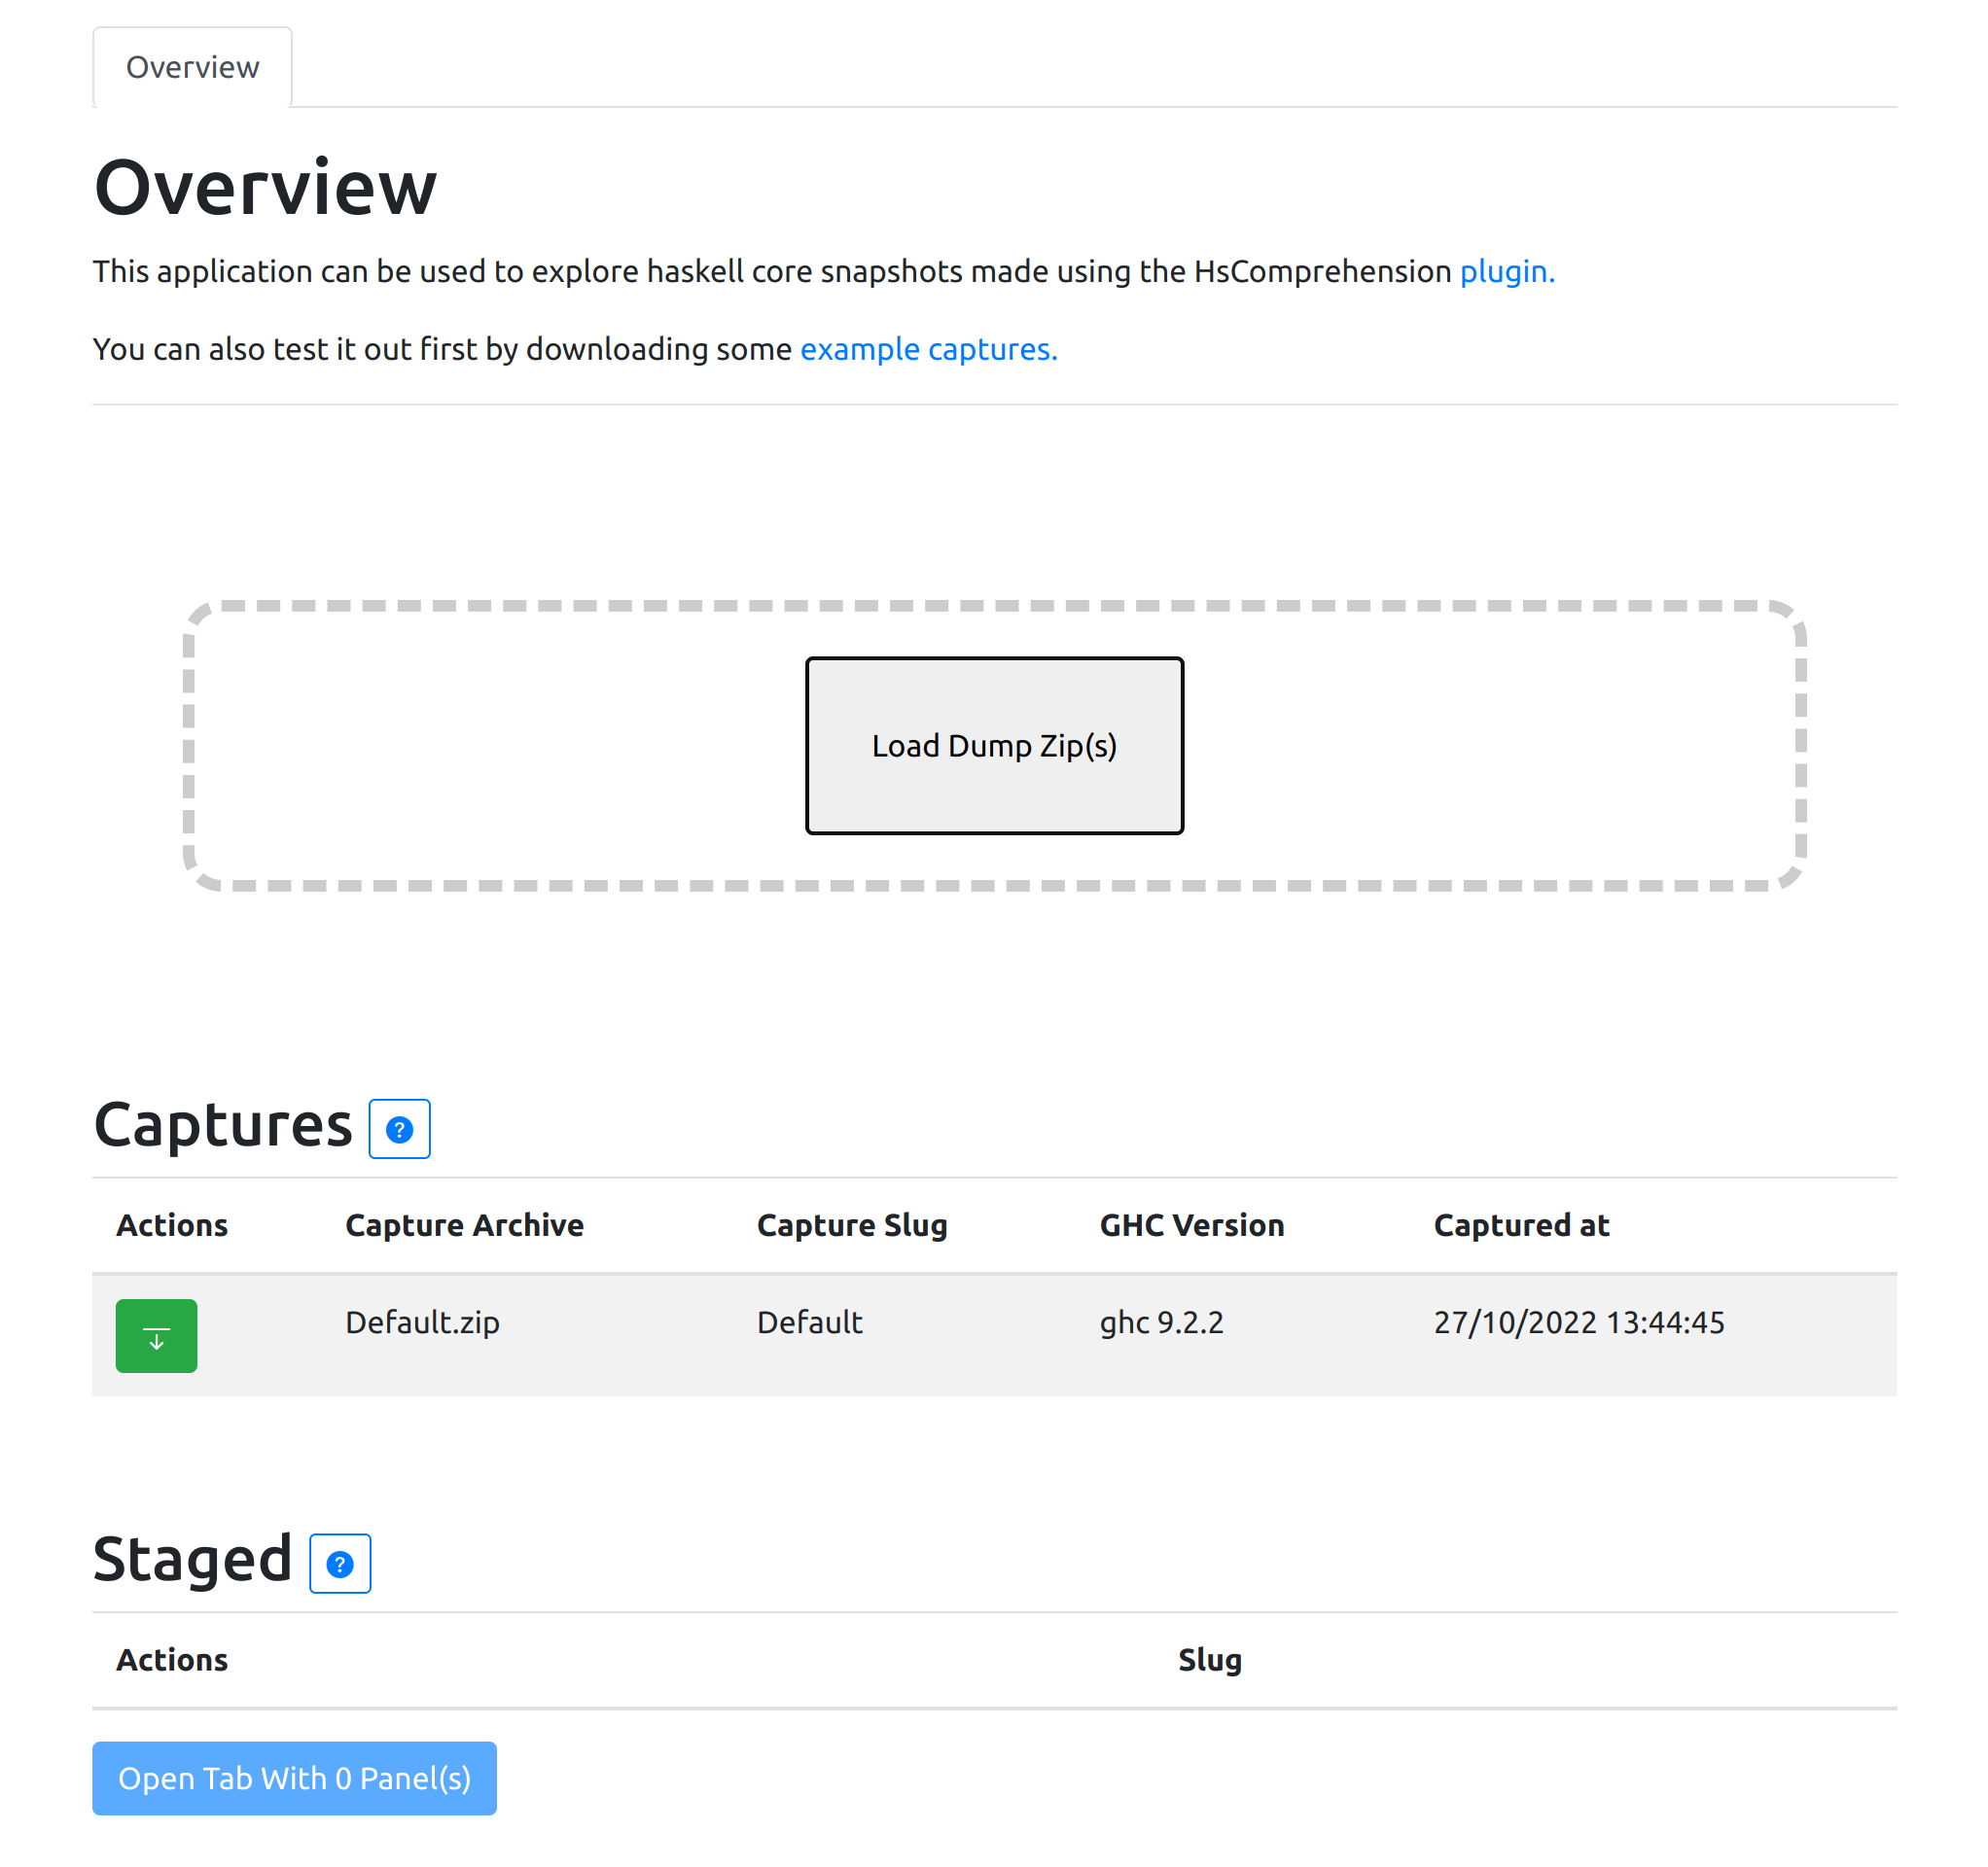
\includegraphics[width=0.8\textwidth]{figs/countchars_1.png}
\label{fig:countchars_1}
\end{figure}

We then click to green arrow to reference the dump in the staging area. Here we could elect to stage more
than one dump if we want to compare them. In this case we just interested in the current situation, and so we
just open a single panel tab with this single dump:


\begin{figure}[H]
\centering
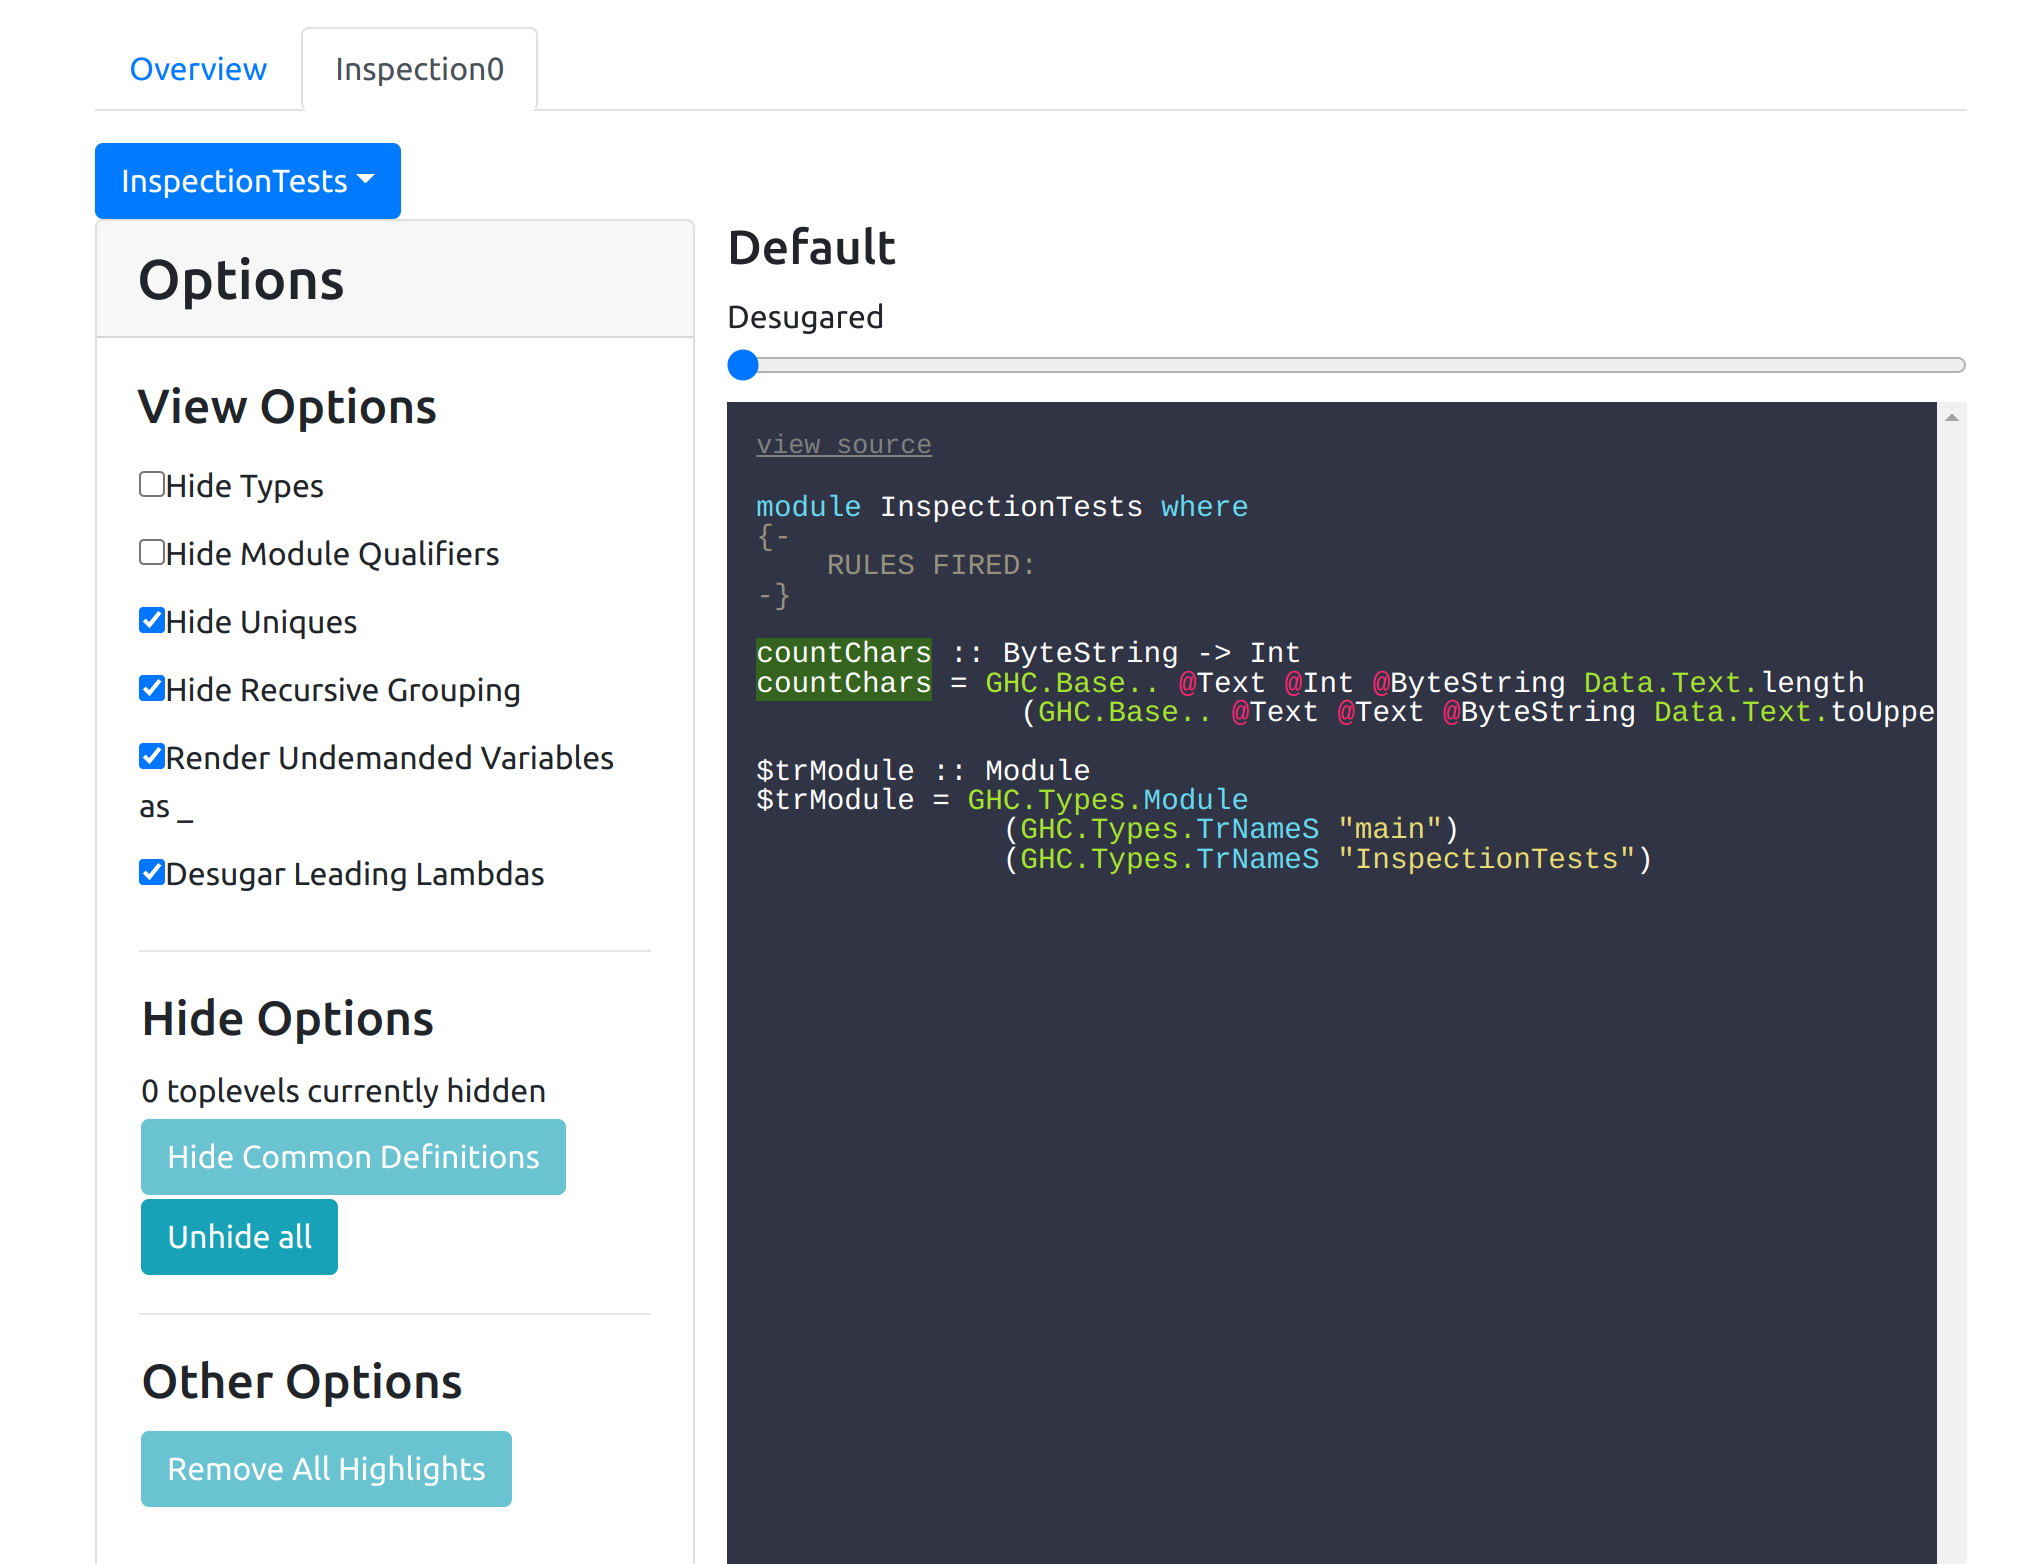
\includegraphics[width=0.8\textwidth]{figs/countchars_2.png}
\label{fig:countchars_2}
\end{figure}

On the left, are immediately presented with a number of viewing options. To the right we can see the rendered
Core, under influence of the view options. Above it a slider indicating that we are looking at the
Core in the desugared stage (so without any transformations yet applied). Scrolling this slider will reveal
the intermediate Core ASTs that were produced by the compiler. Whenever rewrite rules are fired they are included
as comments at the top of the module.

If we scroll all the way to the end, we get the same final Core AST as we saw in the error message. Granted,
we now have syntax highlighting and a slightly more readable representation, but it is still unwieldy. Using
a basic string search we can find the needle in the haystack:

\begin{figure}[H]
\centering
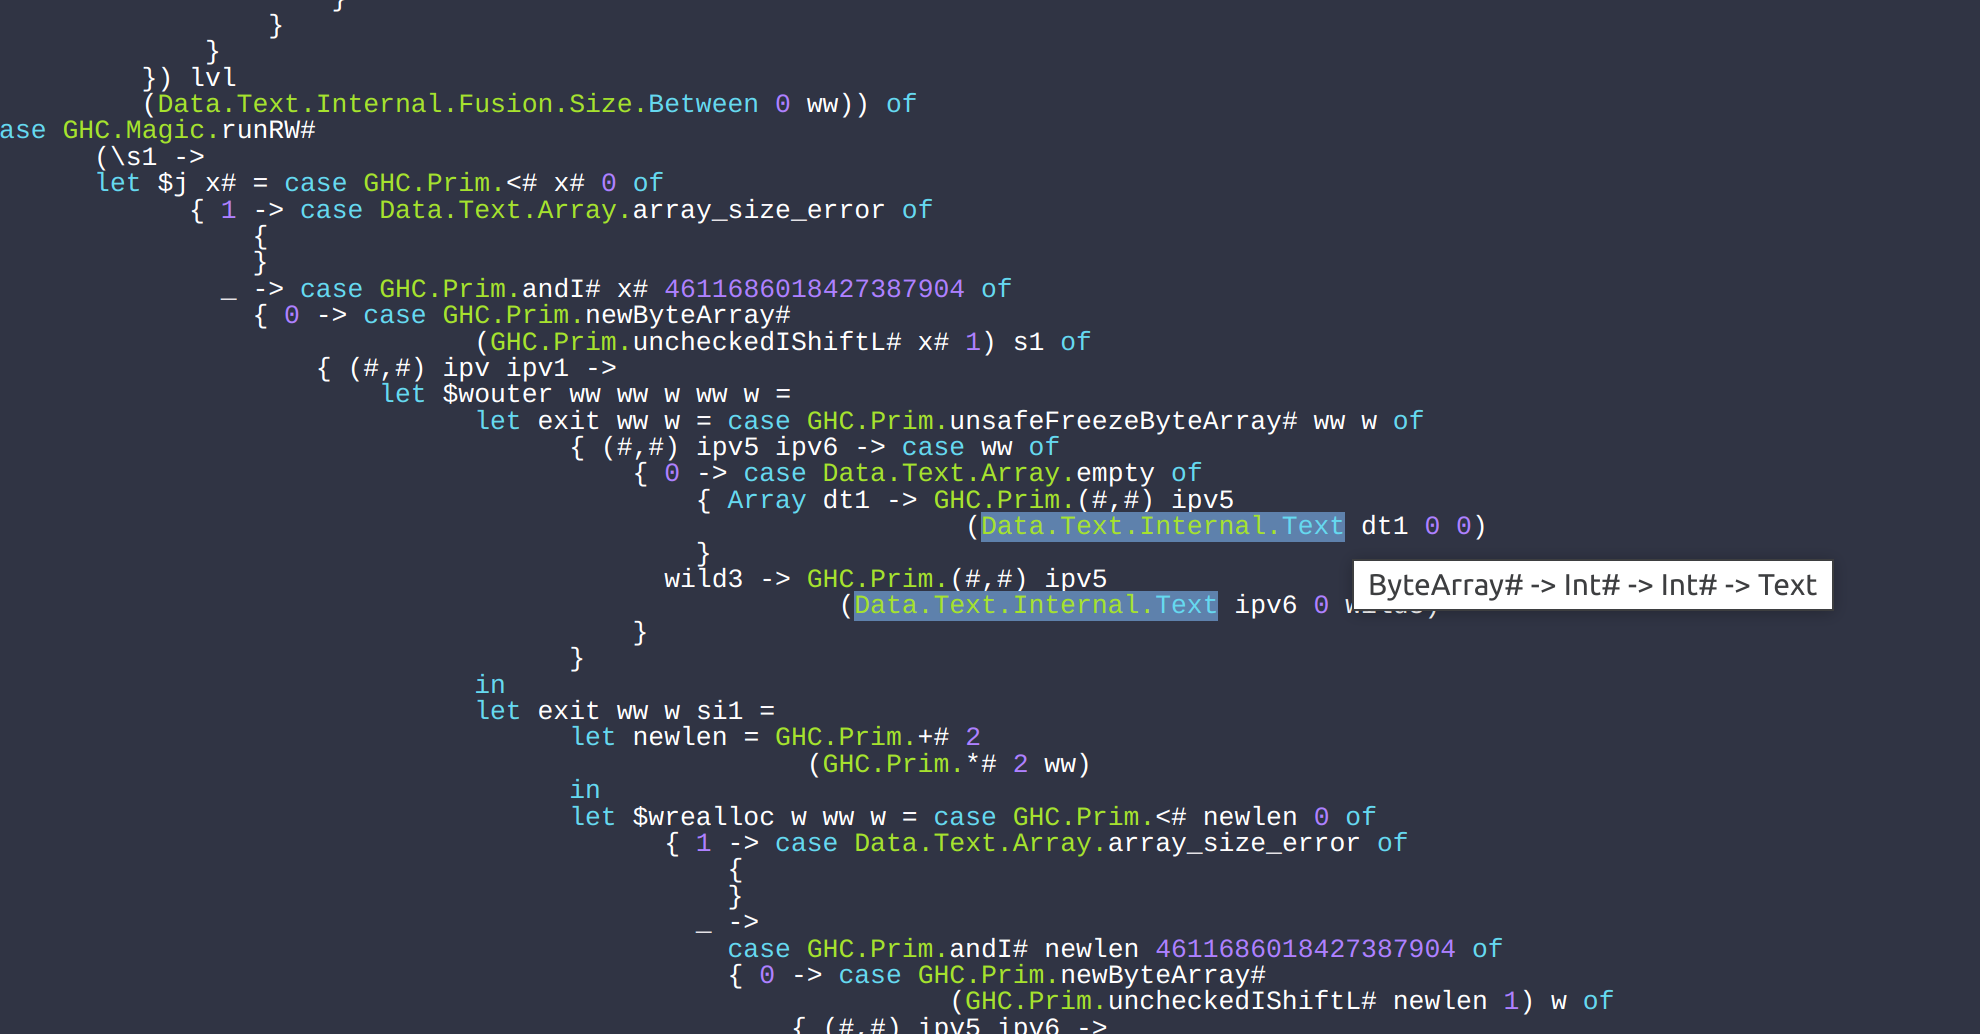
\includegraphics[width=0.8\textwidth]{figs/countchars_3.png}
\end{figure}

But we don't really care about finding the needle, but more so how it got it there.
Using the scroll bar we can go back in time to a moment before everything was inlined.
Specifically, we can go back to the first moment where no \mono{Text} constructor existed yet:

\begin{figure}[H]
\centering
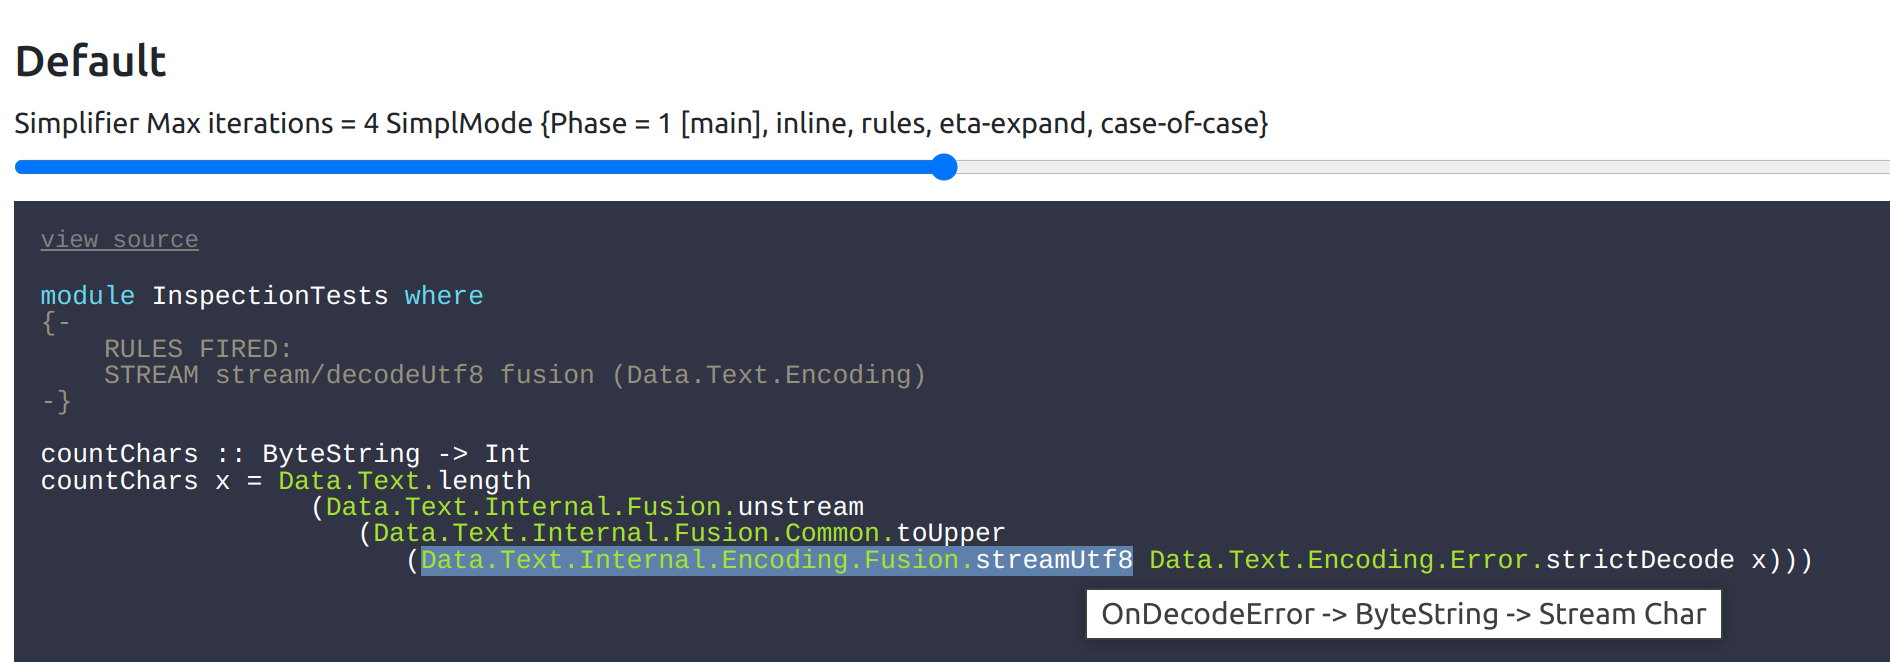
\includegraphics[width=0.8\textwidth]{figs/countchars_4.png}
\end{figure}

We find a far more manageable definition of \mono{countChars} that has partially been transformed to operate on streams (\mono{Stream Char}).
This is a concept based on the work of D. Couts et al. \cite{stream_fusion}, we will discuss its theory more
in depth in next section. For now, it is only important to realise that instead of embedding the
incoming \mono{ByteString} in a \mono{Text} value, we are converting to a \mono{Stream Char} first before \mono{unstream}
converts to an actual \mono{Text}. The argument that this is not necessary still holds because there exists a length
function for values of type \mono{Stream Char} as well. 

So we can conclude that the \mono{text}'s fusion did not fully work as expected because it is conceivable to find the
length of stream directly using some alternative \mono{length :: Stream Char -> Int} function. 

\paragraph{4. Back to the future}

Luckily, we were reliving someone else's experience, and we have the luxury of seeing how the situation unfolded.
So, what we can do is make another capture with a more recent version of the library, and compare the two:

\begin{figure}[H]
\centering
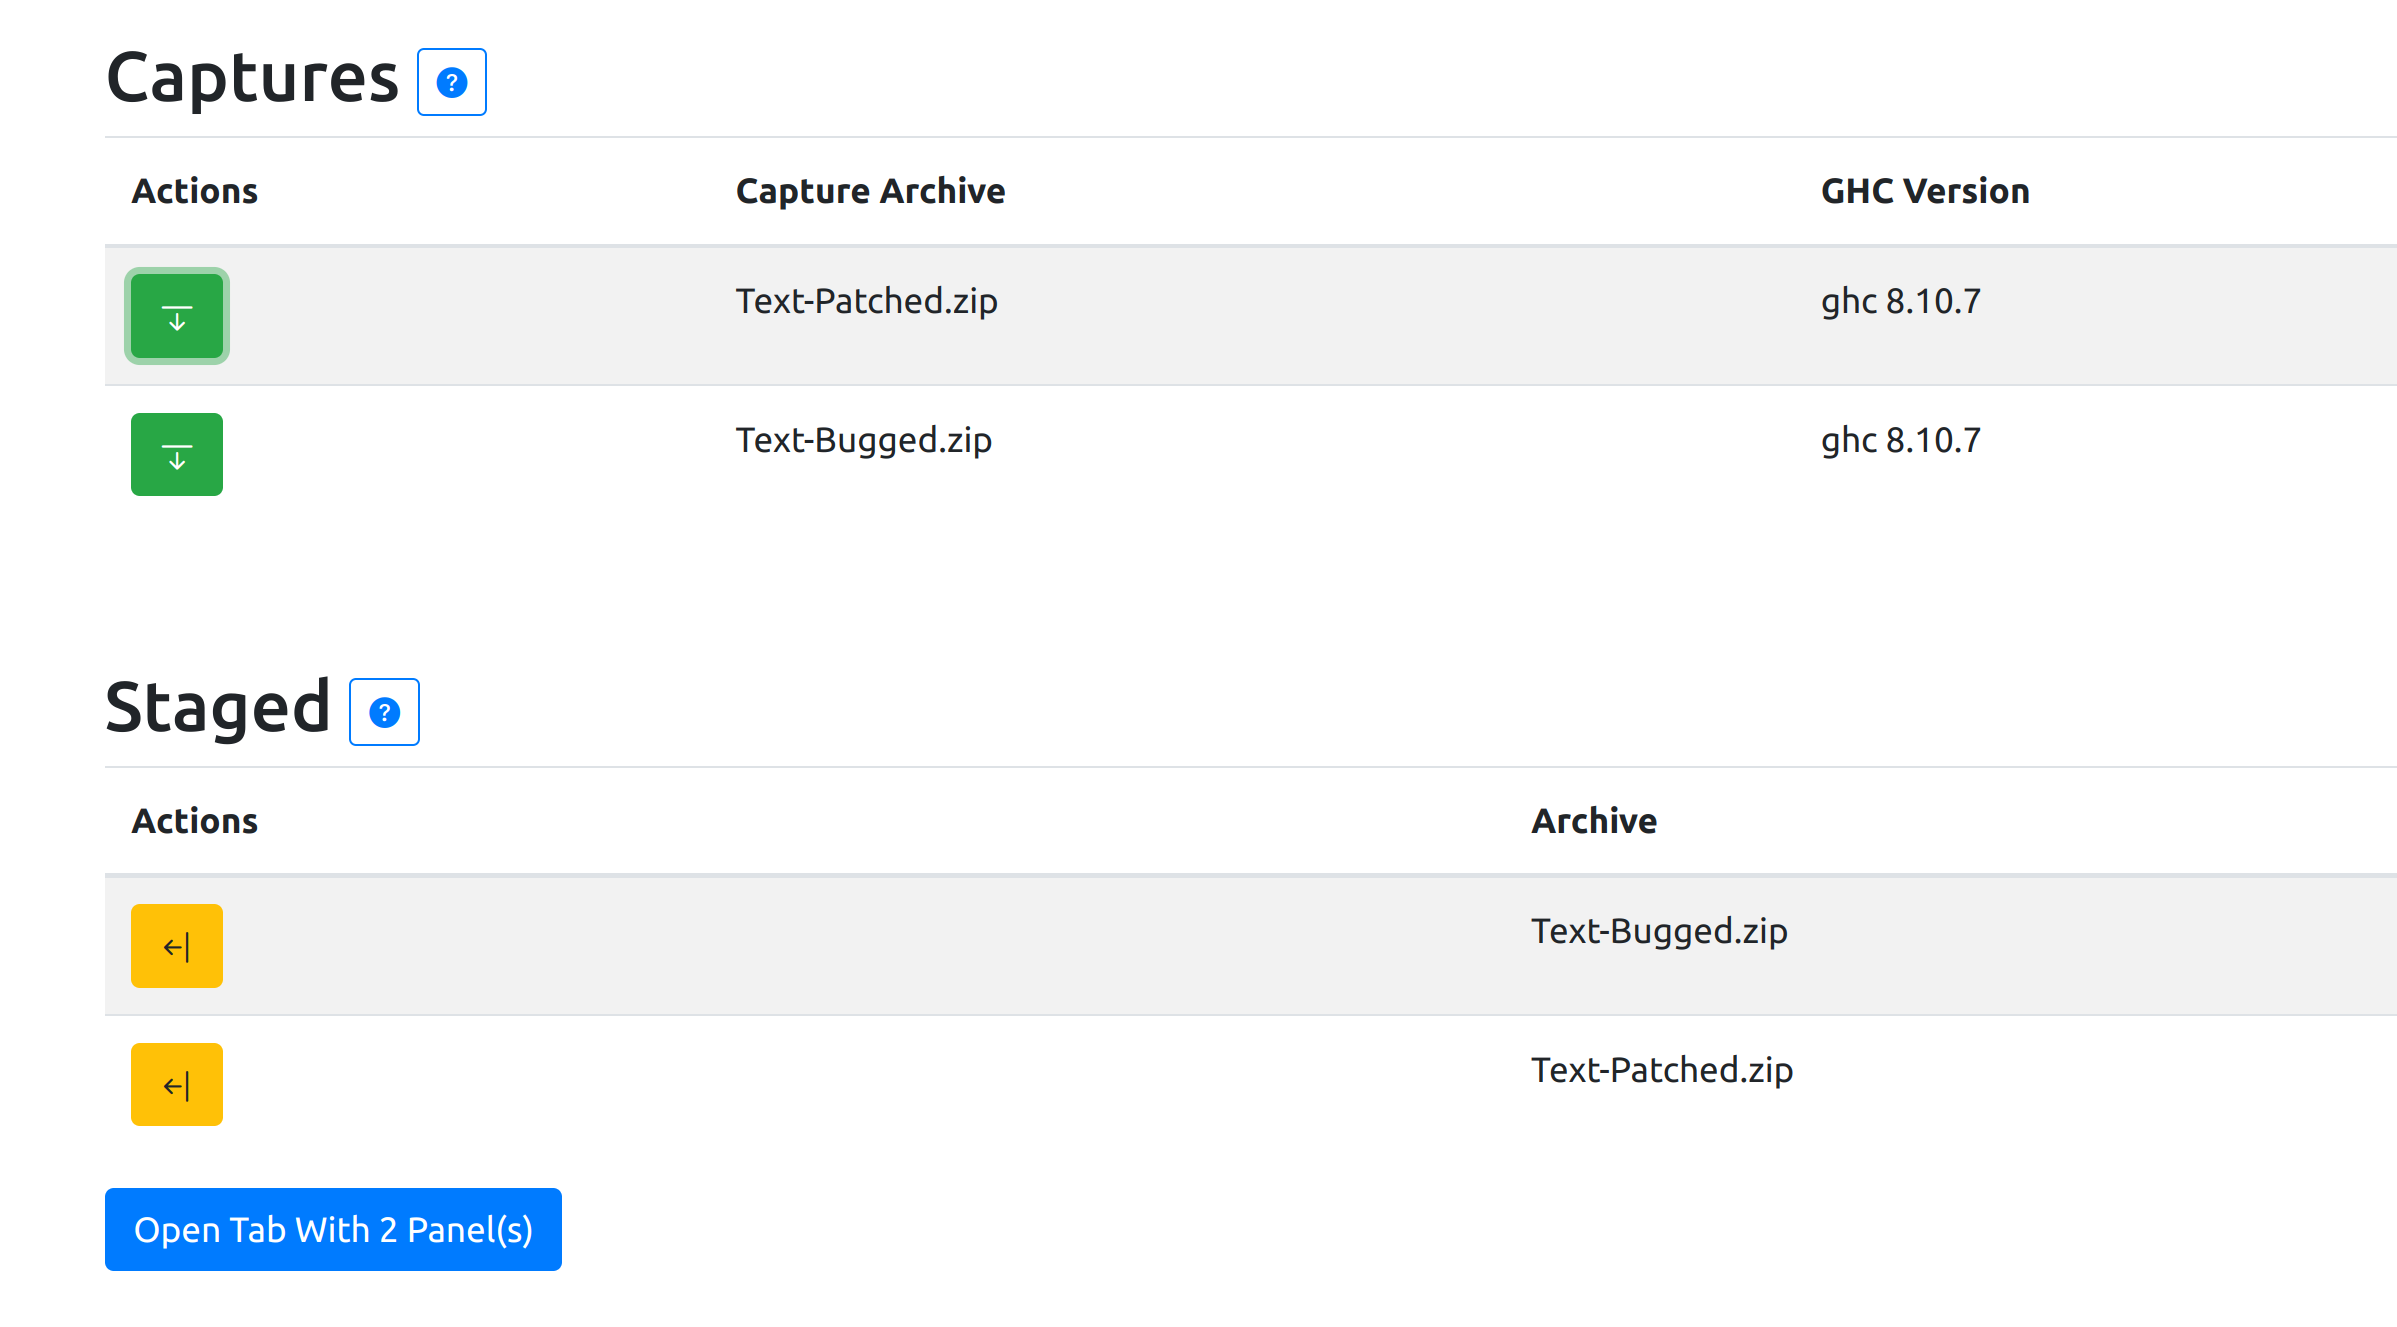
\includegraphics[width=0.8\textwidth]{figs/countchars_5.png}
\end{figure}

Because we now have more than 1 capture open at the same time we can use the \textit{Hide common definitions} feature to
find the first moment where the two captures converge. This happens to be at phase 1 of the simplifier pass:

\begin{figure}[H]
\centering
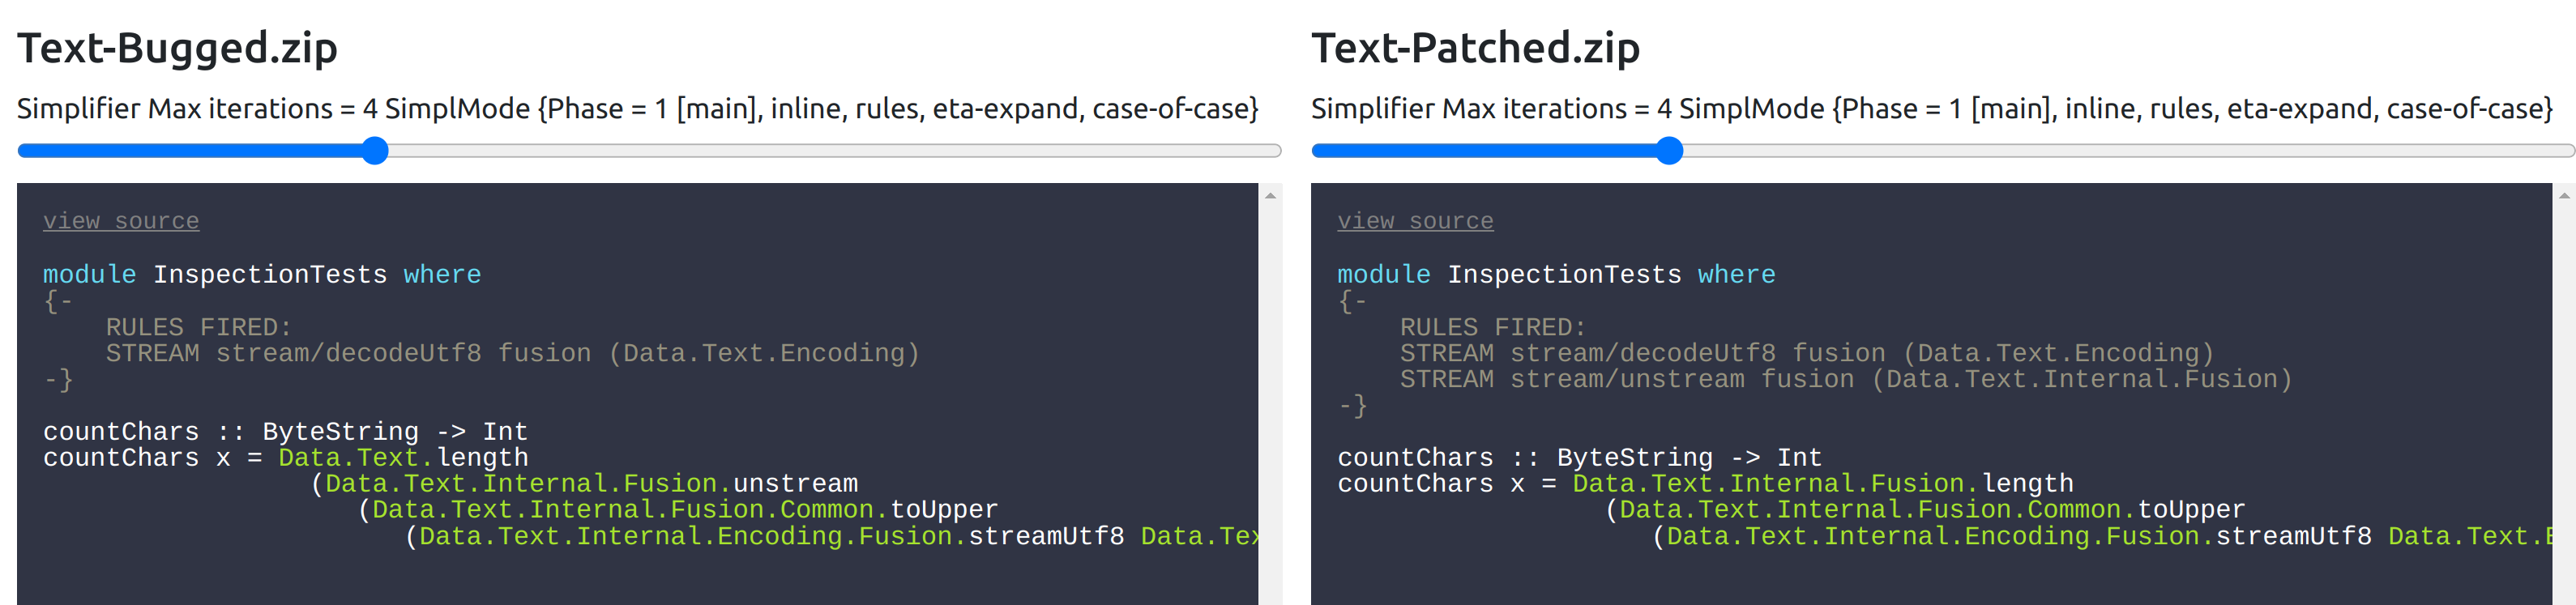
\includegraphics[width=0.9\textwidth]{figs/countchars_6.png}
\end{figure}

For clarity, let us extract the text from the left panel and the right panel and compare them:

\begin{listing}[H]
\begin{minted}[linenos,fontsize=\footnotesize]{haskell}
{-
    Text-Bugged.zip
    RULES FIRED:
    STREAM stream/decodeUtf8 fusion (Data.Text.Encoding)
-}

countChars :: ByteString -> Int
countChars x = Data.Text.length
                 (Data.Text.Internal.Fusion.unstream
                    (Data.Text.Internal.Fusion.Common.toUpper
                       (Data.Text.Internal.Encoding.Fusion.streamUtf8 Data.Text.Encoding.Error.strictDecode x)))

------------------------------------------------------------------
{-
    Text-Patched.zip
    RULES FIRED:
    STREAM stream/decodeUtf8 fusion (Data.Text.Encoding)
    STREAM stream/unstream fusion (Data.Text.Internal.Fusion)
-}

countChars :: ByteString -> Int
countChars x = Data.Text.Internal.Fusion.length
                 (Data.Text.Internal.Fusion.Common.toUpper
                    (Data.Text.Internal.Encoding.Fusion.streamUtf8 Data.Text.Encoding.Error.strictDecode x))
\end{minted}
\end{listing}

The most notable difference is the extra rewrite rule that was fired in the patched version (line 18).
Unfortunately, it is currently not possible to look up the definition of the rewrite rule in the tool itself, but
we are given its name and originating module so, we can find it in the source of \mono{text} without too much effort:

\begin{listing}[H]
\begin{minted}{haskell}
{-# RULES "STREAM stream/unstream fusion" forall s. stream (unstream s) = s #-}
\end{minted}
\end{listing}

From this we learn that at some point there was a stream/unstream pair to remove. Another difference is the origin
of the \mono{length} function (\mono{Data.Text.Internal.Fusion.length} over \mono{Data.Text.length}). Like we predicted earlier,
the patched version uses a variant that operates directly on streams:

\begin{figure}[H]
\centering
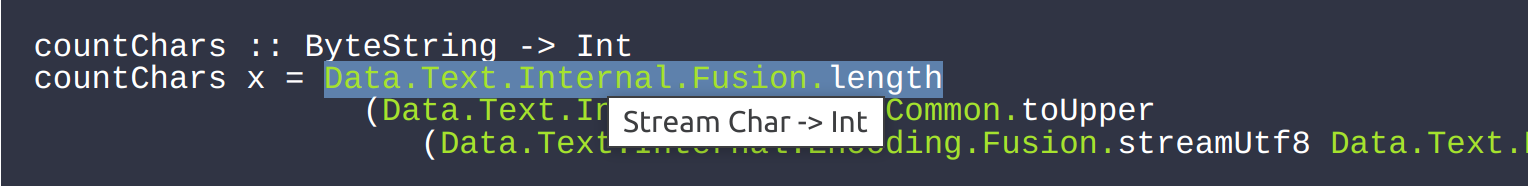
\includegraphics[width=0.8\textwidth]{figs/countchars_7.png}
\end{figure}

Given that in the previous in pass the captures were identical, and since no rewrite rule fired regarding \mono{length},
we can ascribe the difference to the inlining of \mono{length}. If we collect the definition of \mono{length} from both version
of the text library we get:

\begin{listing}[H]
\begin{minted}{haskell}
-- Text-Bugged.zip
length :: Text -> Int
length t = S.length (stream t)
{-# INLINE [0] length #-}

-------------------------------------------

-- Text-Patched.zip
length :: Text -> Int
length t = S.length (stream t)
{-# INLINE [1] length #-}
\end{minted}
\end{listing}

The only difference is the phase annotation of the \mono{INLINE} pragma. The patched version somehow decided that it was better
to inline \mono{length} one simplifier phase earlier (remember, phase 1 comes before phase 0). And they turned out to be right,
because inlining earlier uncovered the opportunity to successfully and remove any occurance of the \mono{Text} constructor.

\paragraph{5. Brittleness of implicit fusion}
At or around the same time as Breitner. \cite{inspection_testing} identified the failed fusion case, Andrew Lelechenko had discovered
a problem involving the \mono{tail} function \cite{two_tails}. \mono{tail} just needs to drop the first character.
Despite needing to check whether to skip 1 or 2 bytes because of the UTF-16 encoding, this can be done in $O(1)$ time and memory.
Obviously this property should still hold when applying \mono{tail} twice in row. As it turns out, it does not. The following steps occur:

\begin{listing}[H]
\begin{minted}{haskell}
tail . tail
-- { inline to fusion variant }
unstream . S.tail . stream . unstream . S.tail . stream
-- { apply 'stream . unstream = id' }
unstream . S.tail . S.tail . stream
\end{minted}
\end{listing}

By constructing a stream we have become committed to traversing the entire structure where it was not needed at first,
yielding an $O(n)$ time and memory version after ``optimisation''. This is different from the situation in \mono{countChars},
where UTF-16 already dictated $O(n)$ runtime.

The ending to this story is quite simply that implicit fusion was disabled entirely \cite{two_tails} for cases where this could occur.
Frequent \mono{text} contributor, Oleg Grenrus, remarked on the proposal to remove it the following:

\textit{``I think this is the right thing to do. Implicit fusion is unpredictable, and you explain, doesn't even work in simple cases.''}

Instead, users can now opt in by using the stream variant of such functions explicitly. This is a tragic example of how optimisation
can be unpredictable, and by extent, how people would favour predictability over automatic performance transformations that risk making the program slower.

\section{Lists vs Streams}

Here we discuss the basic of the stream paper, how it operates, why Haskell has not implemented it by favouring join points and
finally how the compilation pipeline treats these 2.

Perhaps repeat the unlines example from the background section.

% Trying to reach the same conclusion as https://github.com/haskell/text/issues/202 (recursing into the mentioned https://github.com/haskell/text/pull/348)

\section{Performance regression at Channable}

%https://github.com/haskell/text/issues/202
%https://github.com/haskell/text/pull/348
%
%Another performance regression: https://gitlab.haskell.org/ghc/ghc/-/issues/22207

\section{Comparison with existing tools}
